\chapter{State of the art}

\section{Overview}

Three existing solutions for extending Neutron with additional SDN features have been tested. They were selected based on the requirements given in section 3.

\section{OpenDaylight SDN controller}

% %https://www.openstack.org/assets/presentation-media/osodlatl.pdf % %
% %https://github.com/opendaylight/docs/blob/master/manuals/developers-guide/src/main/asciidoc/ovsdb.adoc % %

OpenDaylight is fully implemented in Java. The Controller platform has multiple Northbound \& Southbound interfaces. OpenDaylight exposes a single common OpenStack Service Northbound API which exactly matches the Neutron API. The OpenDaylight OpenStack Neutron Plugin simply passes through and therefore pushes complexity to OpenDaylight and simplifies the OpenStack plugin. The ML2 mechanism driver in Neutron has to be set to the OpenDaylight ML2 plugin with the ODL agent running on the Compute Nodes. The OpenDaylight controller can be run on the Control Node or on a separate VM. The Open vSwitch database (OVSDB) Plugin component for OpenDaylight implements the OVSDB management protocol that allows the southbound configuration of vSwitches. The OpenDaylight controller uses the native OVSDB implementation to manipulate the Open vSwitch database. The component comprises a library and various plugin usages. The OVSDB protocol uses JSON/RPC calls to manipulate a physical or virtual switch that has OVSDB attached to it.

\begin{figure}[H]
\centering
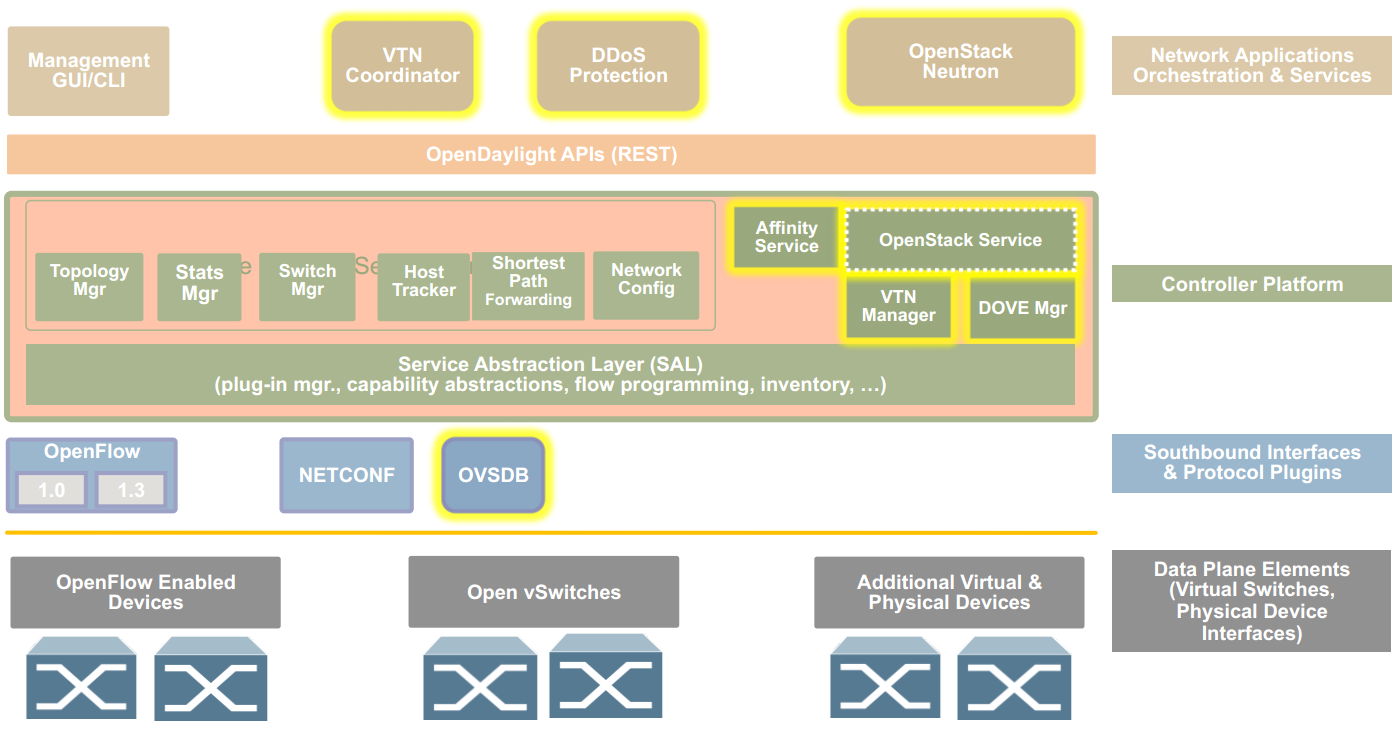
\includegraphics[width=0.9\textwidth]{images/sota/odl_architecture.png}
\caption{Architecture of OpenDaylight Virtualization edition}
\end{figure}

The OVSDB component is accessible through a Northbound ReST API, which enables the operator to connect to the OpenFlow controller and modify various OVSDB tables. Through this API QoS rules can be deployed. Because it connects directly to the OpenVSwitch tables, all the QoS types that come with OpenVSwitch can be deployed (DSCP marking, setting priority, min-/max-rate for switch ports \& OpenFlow Queues). In the local testbed we were able to successfully deploy QoS rules on the ports of Virtual Machines. 


\section{Ryu SDN controller}

% %https://nsrc.org/workshops/2014/nznog-sdn/raw-attachment/wiki/WikiStart/Ryu.pdf % %
% %https://wiki.openstack.org/wiki/Neutron/OFAgent/ComparisonWithOVS % %

Ryu is a component-based software defined networking framework which fully supports OpenFlow 1.0, 1.2, 1.3 and 1.4 switches and is fully written in Python. Ryu is a full featured OpenFlow controller that supports GRE and VLAN tunnelling. The OpenFlow controller that is embedded in the agent sets Flows on the switch by sending OpenFlow messages to the switch. It includes a set of apps which build the base of the SDN controller like L2 switch, ReST interface, topology viewer and tunnel modules. Ryu also includes an app that allows to set QoS rules through a ReST interface which uses a OVSDB interaction library to apply those. The QoS rules can be either applied to a specific Queue within a VLAN or a Switch port. It supports DSCP tagging and setting the min-rate and max-rate of an interface.

\begin{figure}[H]
\centering
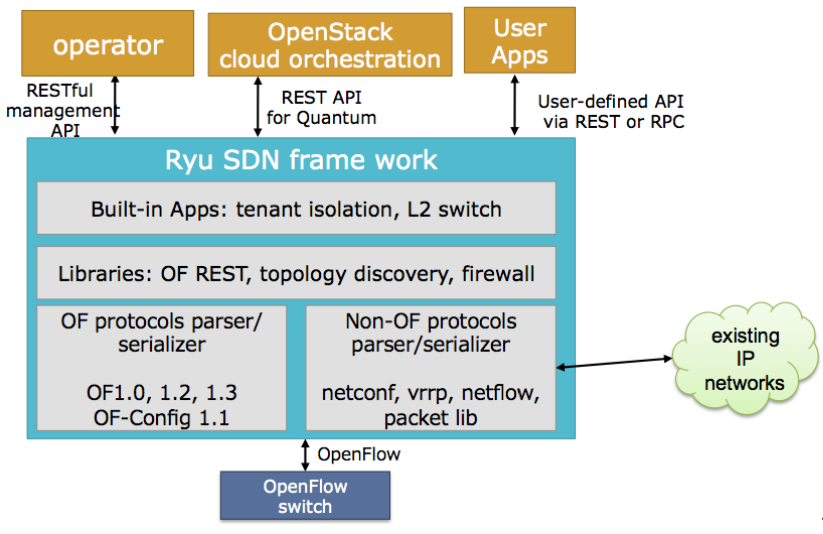
\includegraphics[width=0.7\textwidth]{images/sota/ryu_architecture.png}
\caption{Ryu architecture}
\end{figure}


As of OpenStack IceHouse Ryu has been renamed to OFagent and is included in the Neutron repository. In order to use it as the SDN framework for OpenStack Neutron, OFagent has to be set as both the ML2 mechanism driver (running on the Control / Network node) and the Neutron agent (running on the Compute node). 


\section{OpenStack Neutron - QoS Extension}

% %https://wiki.openstack.org/wiki/Neutron/QoS % %
A Neutron extension has been partially implemented for OpenStack IceHouse which includes an API for setting and retrieving QoS on a per-tenant and per-port basis.

% -> further describe the structure of the implementation !! %

\begin{figure}[H]
\centering
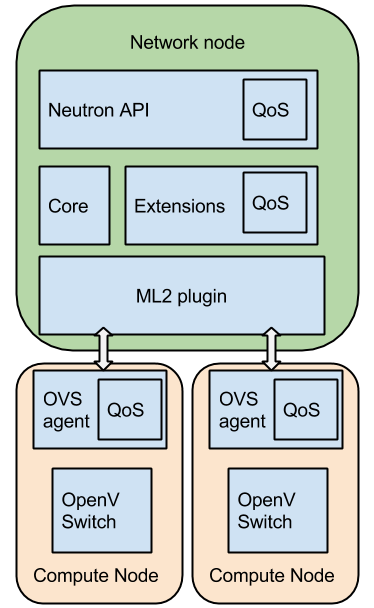
\includegraphics[width=0.3\textwidth]{images/sota/neutron_qos_extension.png}
\caption{Neutron QoS Extension architecture}
\end{figure}



\section{Problem statement}

%Show why previously mentioned projects fail for our requirements, analyse and compare them. Make table with features. Also state that they wouldn't include the VM placement feature. %
This section lists the restrictions that have been discovered with the previously mentioned solutions. 


\textbf{Problems encountered with OpenDaylight:}

The local testbed used for the integration of OpenStack Juno and OpenDaylight Helium consisted of 2 hosts, one running the OpenStack control node and OpenDaylight Controller and a OpenStack Compute Node on the second host. During the tests it was not possible to get the public network access for the Virtual Machines working, thus the L3 routing did not work. This and the fact that it ODL is very complex to debug and understand all underlying processes led us to the decision not to use OpenDaylight.


\textbf{Problems encountered with Ryu:}

The test of Ryu was unsuccessful due to a number of errors while stacking the test environment using Devstack. It was not possible to launch instances and test the QoS features. The lack of proper documentation for the interaction with OpenStack Neutron led us to look more into other SDN controllers for our particular use case. Currently Ryu doesn't support the Distributed Virtual Routing feature that has been introduced with OpenStack Juno.


\textbf{Problems encountered with Neutron QoS Extension:}

The implementation has not been finished and merged into Neutron, however the basic deployment of QoS seem to have been tested successfully. 

At the moment it is not clear if the OpenStack community will keep working on this, according to the whiteboard it was deferred to Juno, but it's not included in the current release and no active development is stated in the code / documentation platforms of the OpenStack community.

The patch consists of an extension to the Neutron API which allows setting QoS rules through the Neutron Python client, the actual Neutron extension with the QoS, QoS Driver in the OpenVSwitch agent and an addition to the Neutron Database that includes QoS.

\section{Conclusion}

The listed problems further strengthen the motivation for the implementation of the Connectivity Manager. A feature comparison and analysis is given.

\begin{tabularx}{\textwidth}{ |X|X|X|X| }
\hline Tool/Solution & QoS support & OF Controller & OpenStack (Juno) integration \\ 
\hline Ryu & X & X & No (tests in Juno failed) \\ 
\hline OpenDaylight & X & X & No (tests in Juno failed) \\ 
\hline Neutron QoS extension & not fully implemented & No & No (IceHouse patch not ported to Juno) \\ 
\hline 
\end{tabularx}
